\documentclass{beamer}

\usepackage{../../presentation}

\title{Walking On Stars \\[1pt] {\Large Grid-less Monte Carlo PDE Solver}}
\author{Yuqi Meng}
\date{Sept. 27, 2024}

\begin{document}

\maketitle

\colortheme{lightgreen}

\section{Spherical Process for the Dirichlet Problem}

\begin{frame}{The Dirichlet Problem}

	\begin{definition}[Harmonic Function]\label{def: harmonic function}
		A twice continuously differentiable $\R$-valued function $u: D \to \R$ is \textbf{harmonic} if $\Delta u := \nabla^2 u \equiv 0$ on $U$.
	\end{definition}
	\horzline

	\begin{definition}[Dirichlet Problem]
		Given a domain (for simplicity assume that this is simply-connected) $D$ with boundary $\partial D$, a \textbf{Dirichlet problem} associated to a function $f$ continuously defined on $\partial D$ is to find the function $u$ defined on $R$ s.t. $u$ and $f$ coincide on $\partial D$, i.e. solve for $u$ s.t.
		\[
			\begin{cases}
				\Delta u = 0, & \text{ on D} \\
				\left. u \right|_{\partial D} = f & \text{(Dirichlet BC)} \\
			\end{cases}
		\]
	\end{definition}
	\horzline

\end{frame}

\begin{frame}{Brownian Motion}

	\begin{definition}[Brownian Motion]
		A \textbf{$\R^d$-valued Brownian motion} starting at $x \in \R^d$ is a stochastic process $\{ B(t) \mid t \in T := \R_{\geq 0} \}$ satisfying the following properties:
		\begin{enumerate}
			\item \emph{Anchor:} $B(0) = x$.
			\item \emph{Independent incrementals:} for any increasing sequence $(t_n)_{n \in \Z_{\geq 0}}$ on $T$, $\{ B(t_{i+1}) - B(t_i) \mid i \in \Z_{\geq 0} \}$ are independent random variables.
			\item \emph{Normality in each step:} For all $t \geq 0, h > 0$, the incremental $B(t + h) - B(t)$ follows a normal distribution $N(0, h)$.
			\item \emph{Continuity:} The function $t \mapsto B(t)$ is almost surely (i.e., has probability 1 of being) continuous.
		\end{enumerate}
	\end{definition}
	\horzline

\end{frame}

\begin{frame}{Kakutani's Principle}

	\begin{theorem}[Kakutani, 1944]
		Given a Dirichlet problem defined on a domain $D$ with boundary values $f(\zeta)$ for $\zeta \in \partial D$, for any $x_0 \in D$, the solution $u$ of the Dirichlet problem evaluates to
    	\[
        	u(x_0) = \int_{\partial D} \Pr(x_0, \zeta, D) f(\zeta) \d \zeta \qquad \forall x_0 \in D
    	\]
    	where $\Pr(x_0, \zeta, D)$ is the probability density function of a Brownian motion starting at $x_0$ intersects for the first time with $\partial D$ at $\zeta$.
	\end{theorem}
	\horzline

	\begin{definition}[Harmonic Measure]
		The measure $\d \omega = \Pr(x_0, \zeta, D) \d \zeta$ on $\partial D$ is the \textbf{harmonic measure}.
	\end{definition}
	\horzline

\end{frame}

\begin{frame}{Kakutani's Principle: Sketch of Idea}

	First verify the simple case, and then extend to general ones:
	\begin{enumerate}
		\item For unit disc, notice that harmonicity is equivalent to ``mean value property'':
        \[
            f(x) = \frac{1}{\abs{\partial \mathcal{S}(x, r)}}\int_{\partial \mathcal{S}(x, r)} f(\zeta) \d \zeta
        \]
		where $\mathcal{S}(x, r)$ is a sphere centered at $x$ with radius $r$.
		\item Then, use the ``local memory-less'' property of Brownian motion to extend to arbitrary closed (nice) domains.
	\end{enumerate}

\end{frame}

\begin{frame}{Spherical Process: Discretizing Brownian Motion}

	\begin{definition}[Maximum Sphere]
		Let $D$ be an arbitrary domain, and $x \in D$ be an arbitrary point. Then the \textbf{maximum sphere} centered at $x$ in $D$, denoted ${K}_D(x)$, is the sphere
		\[
			S(x, \inf_{x_0 \in \partial D} \{ \norm{x - x_0} \})
		\]
		Its boundary (surface of the sphere) is denoted as $\overline{{K}}_D(x)$.
	\end{definition}
	\horzline

	\begin{definition}[Spherical Process (Muller, 1956)]
		Given a domain $D$ with boundary $\partial D$ and an arbitrary point $x \in D$, the \textbf{spherical process} defines a sequence of points $P_n(x, \phi)$ where $\phi$ is the random variable, as follows:
		\begin{enumerate}
			\item $P_0(x, \phi) := x$.
			\item For all $i \in \Z_{\geq 1}$, designate $P_i$ uniformly randomly from $\overline{{K}}_D (P_{i-1})$. 
		\end{enumerate}
	\end{definition}
	\horzline

\end{frame}

\begin{frame}{Spherical Process: Discretizing Brownian Motion}
	
	Notice, that every Brownian motion corresponds to a unique spherical process, and vice versa.

	\begin{enumerate}
		\item[$\Rightarrow$:] Simply record the position where the given Brownian motion for the first time escapes the maximum sphere.
		\item[$\Leftarrow$:] The sphere process terminates with probability 0. Therfore they coincide on (countably) infinite points, and the corresponding time.
	\end{enumerate}

	The argument is flawed with discussion on infinity (but does not interfere with integration).

\end{frame}

\begin{frame}{Monte Carlo Integration}

	\begin{definition}[Monte Carlo Estimator]
		Given a Lebesgue-integrable function $f: D \to \R$, the \textbf{Monte Carlo estimator} for the integral
		\[
			I := \int_D f(x) \d x
		\]
		is the sum
		\[
			\hat{I}_N := \frac{1}{N} \sum_{i = 1}^N \frac{f(x_n)}{p(x_n)}, \qquad x_{(\cdot)} \sim p(\cdot)
		\]
	\end{definition}
	\horzline

	Notice that elementary implementation converges slowly. Cf. bidirectional path tracing for reusing paths.
\end{frame}

\colortheme{lightblue}

\section{Generalizing the Equation}

\begin{frame}{Various Boundary Conditions}

	\begin{definition}
		Given an (ordinary/partial) differential equation with domain $\Omega$,
		\begin{itemize}
			\item A \textbf{Dirichlet boundary condition} fixes the value of solution on the boundary of domain. 
			\item A \textbf{Neumann boundary condition} fixes the derivative (normal) applied at the boundary of the domain.
			\item A \textbf{Robin boundary condition} is a weighed combination of the previous two. Explicitly, for given \emph{functions} $a, b, g$ defined on $\partial \Omega$ the associated Robin boundary condition is (for target function $f$)
			\[
				a\ f + b\ \partial_n f = g \qquad \text{on $\partial \Omega$}
			\]
			where $\partial_n(\cdot)$ denotes the normal derivative.
		\end{itemize}
	\end{definition}
	\horzline

\end{frame}

\begin{frame}{Green Function \& Poisson Kernel}

    \begin{definition}[Green Function]
		Given a domain $D$ with boundary $\partial D$, and a differential operator $\mathcal{L}$, the corresponding \textbf{Green function} $G_x^D(y)$ is defined as the solution to the system
		\[
			\mathcal{L} G_x^D(y) = \delta_x(y)
		\]
		where $\delta_x$ is the dirac delta function with impulse at $x$.
	\end{definition}
	\horzline

	\begin{definition}[Poisson Kernel]
		Under the same setting, the \textbf{Poisson kernel} is the normal derivative of $D$:
		\[
			P_x^D(y) := \frac{ \partial G_x^D(y) }{\partial n_y}
		\]
		where $n_y$ is the normal vector towards the boundary.
	\end{definition}
	\horzline

\end{frame}

\begin{frame}{Generalization of Kakutani's Principle}

	The system then becomes (without Robin BC):
	\[
		\begin{cases}
			\Delta(u) = f, & \text{on $\Omega$} \quad \quad\  \text{(Poisson)} \\
			u = g, & \text{on $\partial \Omega_D$} \quad \text{(Dirichlet)} \\
			\frac{\partial u}{\partial n_{\cdot}} = h, & \text{on $\partial \Omega_N$} \quad \text{(Neumann)} \\
		\end{cases}
	\]

	Integrating and expressing in weak form gives
	\begin{align*}
		u & = \int_{\partial D} P_x^D(z) g(z) \d z & \text{(Dirichlet)}\\
		  & - \int_{\partial D} G_x^D(z) \frac{\partial u(z)}{\partial n_{z}} \d z & \text{(Neumann)} \\
		  & + \int_{D} G_x^D(z) f(z) \d z & \text{(Poisson)}
	\end{align*}

\end{frame}

\begin{frame}{Consistency with Spherical Process}

	For the case of sphere, $G_x^D \equiv 0$, $P_x^D \equiv \frac{1}{\partial B}$. Further setting $f \equiv 0$ we obtain the result by Kakutani:

	\[
		u = \int_{\partial D} \left( \frac{1}{\left| \partial D \right|} \right) g(z) \d z
	\]

\end{frame}

\begin{frame}{Outline of Generalization}
	Extending from Dirichlet BC for the Dirichlet problem to arbitrary BC for any PDE, the algorithm needs to be modified in the following aspects:
	\begin{itemize}
		\item Generalize Kakutani's principle, taking into consideration of arbitrary differential operators.
		\item Use different boundary treatments (for Dirichlet BC, this is just terminating the walk).
		\item Generalize the Spherical Process to ensure convergence.
	\end{itemize}
\end{frame}

\colortheme{lightpurple}

\section{Boundary Treatments}

\begin{frame}{Analogy of Boundary Conditions}

	Think in terms of rendering, we have the natural analogy of BCs:
	\begin{enumerate}
		\item Dirichlet BC fixes the value, can be regarded as the \emph{light source}.
		\item Neumann BC fixes the normal derivative, can be regarded as \emph{reflection}.
		\item Robin BC mixes the two above, can be regarded as the \emph{specular/diffusion coefficient}.
	\end{enumerate}

	This naturally inspires the following treatment (rigorous proof will not be simple).

\end{frame}

\begin{frame}{Dirichlet BC}

	Following the previous reduction to spherical process, the Monte Carlo integrator terminates at Dirichlet BCs:
	
	\begin{figure}[htbp]
		\centering
		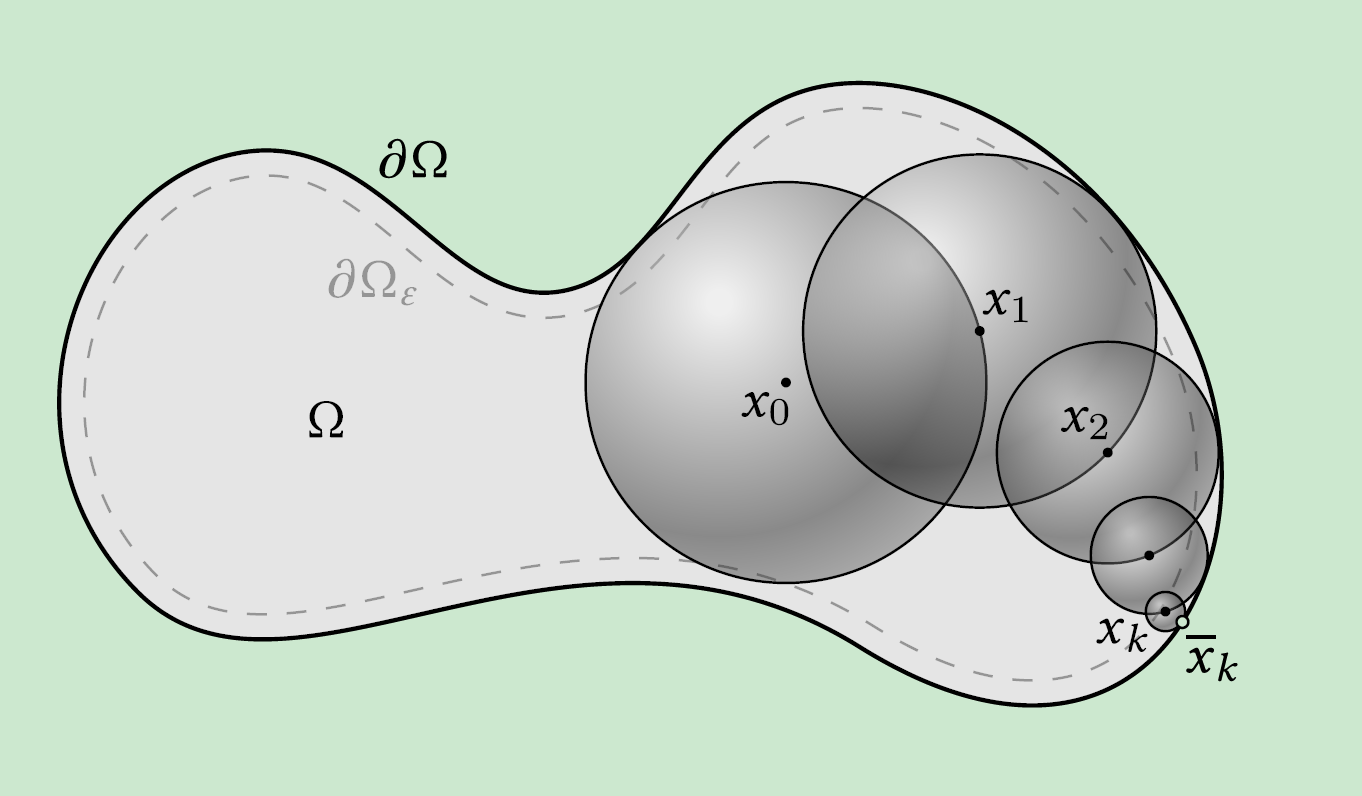
\includegraphics[scale=0.3]{img/DBC.png}
	\end{figure}


\end{frame}

\begin{frame}{Neumann BC: Intuitive approach}
	
	Notice: Neumann BC alone cannot fix a solution.

	The intuitive approach would be to let sample points ``bounce back'' in the normal direction to only capture the tangential component. However, this will cause instabilities..

	\begin{figure}[htbp]
		\centering
		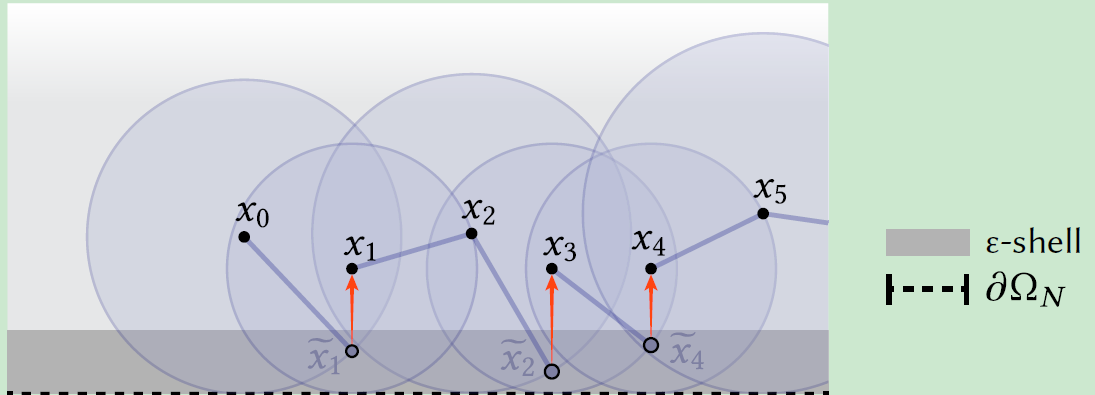
\includegraphics[scale=0.4]{img/NBC-1.png}
	\end{figure}

\end{frame}

\begin{frame}{Neumann BC: Update Scheme}

	Change: set radius to minimum of distance to Dirichlet boundary, and distance to ``silhouette'' points: 

	\begin{figure}[htbp]
		\centering
		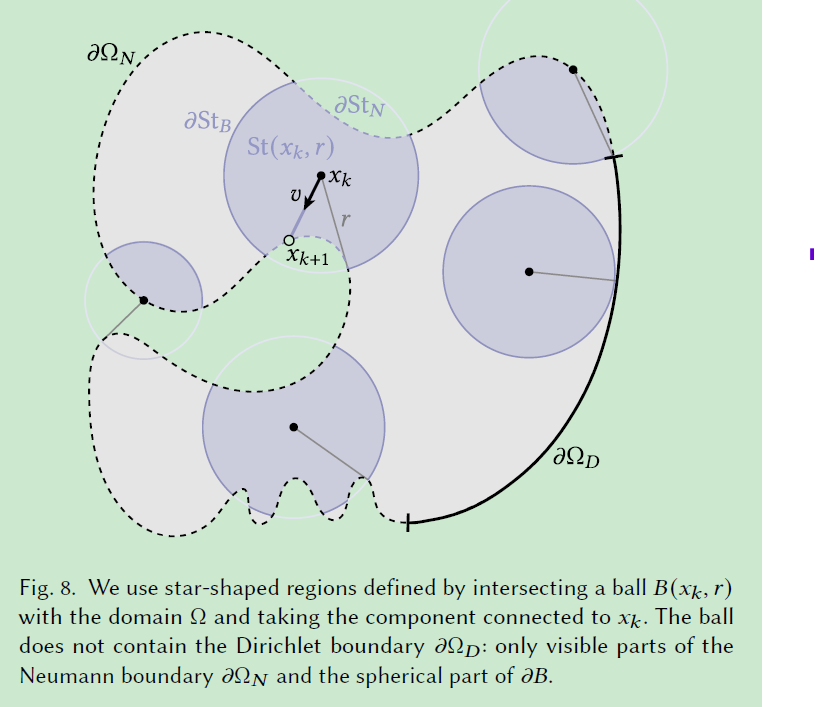
\includegraphics[scale=0.4]{img/NBC-2.png}
	\end{figure}

\end{frame}

\begin{frame}{Neumann BC: Update Scheme}

	The silhouette points are defined to avoid divergence:
	\begin{figure}[htbp]
		\centering
		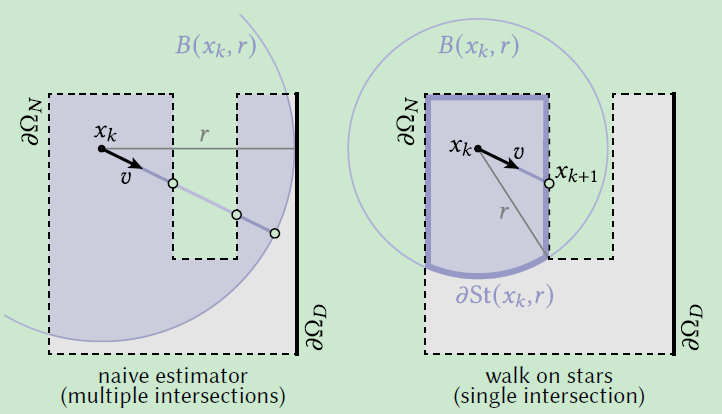
\includegraphics[scale=0.4]{img/NBC-3.png}
	\end{figure}
	Radius update is set in random direction, and intersection with Neumann part first, then spherical part.

	\vspace*{1em}
	\emph{Many intricate details here.}

\end{frame}

\begin{frame}{Robin BC}

	Natural thought: blend between Dirichlet BC and Neumann BC.

	\vspace*{1em}
	High level idea: mimic the solution to path tracing. Interpolate between the radius for pure Dirichlet and pure Neumann for radius update, and apply Russian Roulette for early termination. This is possible as Robin BC contains information about Dirichlet BC.
\end{frame}

\begin{frame}{The Series of Works}
	Foundation: 

	Monte Carlo Geometry Processing: A Grid-Free Approach to PDE-Based Methods on Volumetric Domains (2020)

	Subsequent Works:
	% \vspace*{-0.5em}
	\begin{figure}
		\centering
		
\includegraphics[scale=0.25]{img/related-works.png}
	\end{figure}
\end{frame}

% \colortheme{grey}

% \section{Applied Approaches}

% \begin{frame}{Sample Frame}

% 	Applied stuff.

% \end{frame}

\colortheme{default}

\thankframe

\end{document}
